% !TEX program = xelatex
\documentclass[]{article}
\usepackage{commons/course}

\begin{document}
\printheader

\section*{سوال اول}
\subsection*{قسمت اول}
برای خط 14 داریم:
\begin{latin}
\centering
\begin{tabular}{|c|c|c|c|}
    \hline
    Index & Lexeme & Type & Attributes\\
    \hline
    1 & P & Program Definition & \\
    2 & a & real & \\
    3 & Q & Procedure & \\
    4 & i & int & \\
    5 & b & int array & 1-D, 10 elements \\
    6 & R & Procedure & \\
    7 & d & int & \\
    8 & a & int & \\
    9 & c & int array & 1-D, 5 elements \\
    10 & T & Procedure & \\
    11 & j & real & \\
    12 & d & real & \\
    \hline
\end{tabular}
\begin{tabular}{|c|}
    \hline
    Scope Stack\\
    \hline
    0\\
    \hline
    4\\
    \hline
    7\\
    \hline
    11\\
    \hline
\end{tabular}
\end{latin}
برای خط 19 داریم:
\begin{latin}
\centering
\begin{tabular}{|c|c|c|c|}
    \hline
    Index & Lexeme & Type & Attributes\\
    \hline
    1 & P & Program Definition & \\
    2 & a & real & \\
    3 & Q & Procedure & \\
    4 & i & int & \\
    5 & b & int array & 1-D, 10 elements \\
    6 & S & Procedure & \\
    7 & d & real & \\
    \hline
\end{tabular}
\begin{tabular}{|c|}
    \hline
    Scope Stack\\
    \hline
    0\\
    \hline
    4\\
    \hline
    7\\
    \hline
\end{tabular}
\end{latin}
\subsection*{قسمت دوم}
\begin{enumerate}
    \item در خط 6 ممکن است که به خطای \lr{index out of bounds} بر بخوریم.
    \item در خط 10 نیز دقیقا همین مشکل وجود دارد.
    \item در خط 14 نیز دقیقا همین \lr{dynamic error} ممکن است که به وجود بیاید.
    \item در خط 6 ممکن است که بخاطر جمع کردن یک real با int و ریختن آن در یک آرایه int خطای cast به وجود بیاید. (\lr{type error})
    \item مشکل ذکر شده در خط 11 نیز وجود دارد.
\end{enumerate}
\section*{سوال دوم}
می‌توان این قانون را به صورت زیر نوشت:
\begin{latin}
    \centering
    F $\rightarrow$ \textbf{do} \texttt{\#allocate\_result} E \texttt{\#true\_case} \textbf{if} E \texttt{\#condition} \textbf{else} E \texttt{\#exited} \textbf{fi}
\end{latin}
هر کدام از
\lr{action}ها
را به صورت زیر تعریف می‌کنیم:
\codesample{codes/action-definition.txt}
سعی کردم که در خود کد با کامنت توضیح بدهم که چرا هر خط نوشته شده است. همچنین در اینجا اولین
متغیر در هر دستور عملا نتیجه دستور است. (مثل سینتکس اسمبلی اینتل)

حال ورودی داده شده را پارس می‌کنیم. فرض کنید که
\lr{symbol table}
به صورت زیر است:
\begin{latin}
\centering
\begin{tabular}{|c|c|c|}
    \hline
    Lexeme & Address\\
    \hline
    a & 100\\
    b & 101\\
    e & 102\\
    c & 103\\
    d & 104\\
    h & 105\\
    \hline
\end{tabular}
\end{latin}
در ادامه برای دستور‌ها تا زمانی که به اولین
action
که خودمان اضافه کردیم داریم:
\begin{latin}
\centering
\begin{tabular}{|c|c|c|}
    \hline
    i & PB[i] & Semantic Action\\
    \hline
    0 & (+, 500 a, b) & \#add\\
    \hline
\end{tabular}
\begin{tabular}{|c|}
    \hline
    Semantic Stack (bottom to top)\\
    \hline
    501 (address of result of \textbf{do if})\\
    \hline
    500 (address of a + b)\\
    \hline
\end{tabular}
\end{latin}
حال با رسیدن به
\lr{\#true\_case}
آدرس جواب
\lr{(5 + e)}
در استک است.
\begin{latin}
\centering
\begin{tabular}{|c|c|c|}
    \hline
    i & PB[i] & Semantic Action\\
    \hline
    0 & (+, 500 a, b) & \#add\\
    1 & (+, 502, \#5, e) & \#add\\
    \hline
\end{tabular}
\begin{tabular}{|c|}
    \hline
    Semantic Stack (bottom to top)\\
    \hline
    502 (address of e + 5)\\
    \hline
    501 (address of result of \textbf{do if})\\
    \hline
    500 (address of a + b)\\
    \hline
\end{tabular}
\end{latin}
و بعد از اجرای آن داریم:
\begin{latin}
\centering
\begin{tabular}{|c|c|c|}
    \hline
    i & PB[i] & Semantic Action\\
    \hline
    0 & (+, 500 a, b) & \#add\\
    1 & (+, 502, \#5, e) & \#add\\
    2 & (:=, 501, 502) & \#true\_case\\
    \hline
\end{tabular}
\begin{tabular}{|c|}
    \hline
    Semantic Stack (bottom to top)\\
    \hline
    501 (address of result of \textbf{do if})\\
    \hline
    500 (address of a + b)\\
    \hline
\end{tabular}
\end{latin}
حال خود شرط تبدیل به کد می‌شود که باعث می‌شود که بعد از اجرای
\lr{\#condition}
به حالت زیر برسیم:
\begin{latin}
\centering
\begin{tabular}{|c|c|c|}
    \hline
    i & PB[i] & Semantic Action\\
    \hline
    0 & (+, 500 a, b) & \#add\\
    1 & (+, 502, \#5, e) & \#add\\
    2 & (:=, 501, 502) & \#true\_case\\
    3 & (+, 503, c, d) & \#add\\
    4 & ? & \#condition\\
    \hline
\end{tabular}
\begin{tabular}{|c|}
    \hline
    Semantic Stack (bottom to top)\\
    \hline
    4 (to be backpatched)\\
    \hline
    503 (address of c + d)\\
    \hline
    501 (address of result of \textbf{do if})\\
    \hline
    500 (address of a + b)\\
    \hline
\end{tabular}
\end{latin}
حال وارد یک
\textbf{do}
دیگر می‌شویم. پس داریم:
\begin{latin}
\centering
\begin{tabular}{|c|c|c|}
    \hline
    i & PB[i] & Semantic Action\\
    \hline
    0 & (+, 500 a, b) & \#add\\
    1 & (+, 502, \#5, e) & \#add\\
    2 & (:=, 501, 502) & \#true\_case\\
    3 & (+, 503, c, d) & \#add\\
    4 & ? & \#condition\\
    \hline
\end{tabular}
\begin{tabular}{|c|}
    \hline
    Semantic Stack (bottom to top)\\
    \hline
    504 (address of result of \textbf{do if})\\
    \hline
    4 (to be backpatched)\\
    \hline
    503 (address of c + d)\\
    \hline
    501 (address of result of \textbf{do if})\\
    \hline
    500 (address of a + b)\\
    \hline
\end{tabular}
\end{latin}
سپس دوباره به ترتیب داریم:
\begin{latin}
\centering
\begin{tabular}{|c|c|c|}
    \hline
    i & PB[i] & Semantic Action\\
    \hline
    0 & (+, 500 a, b) & \#add\\
    1 & (+, 502, \#5, e) & \#add\\
    2 & (:=, 501, 502) & \#true\_case\\
    3 & (+, 503, c, d) & \#add\\
    4 & ? & \#condition\\
    5 & (*, 505 3, a) & \#mult\\
    6 & (:=, 504, 505) & \#true\_case\\
    \hline
\end{tabular}
\begin{tabular}{|c|}
    \hline
    Semantic Stack (bottom to top)\\
    \hline
    504 (address of result of \textbf{do if})\\
    \hline
    4 (to be backpatched)\\
    \hline
    503 (address of c + d)\\
    \hline
    501 (address of result of \textbf{do if})\\
    \hline
    500 (address of a + b)\\
    \hline
\end{tabular}
\end{latin}
\begin{latin}
\centering
\begin{tabular}{|c|c|c|}
    \hline
    i & PB[i] & Semantic Action\\
    \hline
    0 & (+, 500 a, b) & \#add\\
    1 & (+, 502, \#5, e) & \#add\\
    2 & (:=, 501, 502) & \#true\_case\\
    3 & (+, 503, c, d) & \#add\\
    4 & ? & \#condition\\
    5 & (*, 505, \#3, a) & \#mult\\
    6 & (:=, 504, 505) & \#true\_case\\
    7 & (+, 506, \#5, h) & \#add\\
    8 & ? & \#condition\\
    \hline
\end{tabular}
\begin{tabular}{|c|}
    \hline
    Semantic Stack (bottom to top)\\
    \hline
    8 (to be backpatched)\\
    \hline
    506 (address of 5 + h)\\
    \hline
    504 (address of result of \textbf{do if})\\
    \hline
    4 (to be backpatched)\\
    \hline
    503 (address of c + d)\\
    \hline
    501 (address of result of \textbf{do if})\\
    \hline
    500 (address of a + b)\\
    \hline
\end{tabular}
\end{latin}
حال در ادامه
\lr(b + c)
تبدیل به کد می‌شود. در اینجا متغیر‌های کامپایلر به صورت زیر در می‌آید:
\begin{latin}
\centering
\begin{tabular}{|c|c|c|}
    \hline
    i & PB[i] & Semantic Action\\
    \hline
    0 & (+, 500 a, b) & \#add\\
    1 & (+, 502, \#5, e) & \#add\\
    2 & (:=, 501, 502) & \#true\_case\\
    3 & (+, 503, c, d) & \#add\\
    4 & ? & \#condition\\
    5 & (*, 505, \#3, a) & \#mult\\
    6 & (:=, 504, 505) & \#true\_case\\
    7 & (+, 506, \#5, h) & \#add\\
    8 & ? & \#condition\\
    9 & (+, 507, b, c) & \#add\\
    \hline
\end{tabular}
\begin{tabular}{|c|}
    \hline
    Semantic Stack (bottom to top)\\
    \hline
    507 (address of 5 + h)\\
    \hline
    8 (to be backpatched)\\
    \hline
    506 (address of 5 + h)\\
    \hline
    504 (address of result of \textbf{do if})\\
    \hline
    4 (to be backpatched)\\
    \hline
    503 (address of c + d)\\
    \hline
    501 (address of result of \textbf{do if})\\
    \hline
    500 (address of a + b)\\
    \hline
\end{tabular}
\end{latin}
سپس به اولین
\lr{exited}
می‌رسیم که باعث می‌شود به صورت زیر در بیاید:
\begin{latin}
\centering
\begin{tabular}{|c|c|c|}
    \hline
    i & PB[i] & Semantic Action\\
    \hline
    0 & (+, 500 a, b) & \#add\\
    1 & (+, 502, \#5, e) & \#add\\
    2 & (:=, 501, 502) & \#true\_case\\
    3 & (+, 503, c, d) & \#add\\
    4 & ? & \#condition\\
    5 & (*, 505, \#3, a) & \#mult\\
    6 & (:=, 504, 505) & \#true\_case\\
    7 & (+, 506, \#5, h) & \#add\\
    8 & (jpt, 506, 11) & \#condition\\
    9 & (+, 507, b, c) & \#add\\
    10 & (:=, 504, 507) & \#exited\\
    \hline
\end{tabular}
\begin{tabular}{|c|}
    \hline
    Semantic Stack (bottom to top)\\
    \hline
    504 (address of result of \textbf{do if})\\
    \hline
    4 (to be backpatched)\\
    \hline
    503 (address of c + d)\\
    \hline
    501 (address of result of \textbf{do if})\\
    \hline
    500 (address of a + b)\\
    \hline
\end{tabular}
\end{latin}
حال همان طور که مشخص است نتیجه در خانه‌ی 504 ذخیره شده است. حال به دومین
\lr{\#exited}
می‌رسیم (برای \textbf{\lr{do if}} بیرونی)
که باعث می‌شود تغییرات زیر اعمال بشود:
\begin{latin}
\centering
\begin{tabular}{|c|c|c|}
    \hline
    i & PB[i] & Semantic Action\\
    \hline
    0 & (+, 500 a, b) & \#add\\
    1 & (+, 502, \#5, e) & \#add\\
    2 & (:=, 501, 502) & \#true\_case\\
    3 & (+, 503, c, d) & \#add\\
    4 & (jpt, 506, 12) & \#condition\\
    5 & (*, 505, \#3, a) & \#mult\\
    6 & (:=, 504, 505) & \#true\_case\\
    7 & (+, 506, \#5, h) & \#add\\
    8 & (jpt, 506, 11) & \#condition\\
    9 & (+, 507, b, c) & \#add\\
    10 & (:=, 504, 507) & \#exited\\
    11 & (:=, 501, 504) & \#exited\\
    \hline
\end{tabular}
\begin{tabular}{|c|}
    \hline
    Semantic Stack (bottom to top)\\
    \hline
    501 (address of result of \textbf{do if})\\
    \hline
    500 (address of a + b)\\
    \hline
\end{tabular}
\end{latin}
در نهایت نیز صرفا دو ضرب دیگر اجرا می‌شود و کد نهایی به صورت زیر است:
\begin{latin}
\centering
\begin{tabular}{|c|c|c|}
    \hline
    i & PB[i] & Semantic Action\\
    \hline
    0 & (+, 500 a, b) & \#add\\
    1 & (+, 502, \#5, e) & \#add\\
    2 & (:=, 501, 502) & \#true\_case\\
    3 & (+, 503, c, d) & \#add\\
    4 & (jpt, 506, 12) & \#condition\\
    5 & (*, 505, \#3, a) & \#mult\\
    6 & (:=, 504, 505) & \#true\_case\\
    7 & (+, 506, \#5, h) & \#add\\
    8 & (jpt, 506, 11) & \#condition\\
    9 & (+, 507, b, c) & \#add\\
    10 & (:=, 504, 507) & \#exited\\
    11 & (:=, 501, 504) & \#exited\\
    12 & (*, 508, 500, 501) & \#mult\\
    13 & (+, 509, h, \#3) & \#add\\
    14 & (*, 510, 508, 509) & \#mult\\
    \hline
\end{tabular}
\begin{tabular}{|c|}
    \hline
    Semantic Stack (bottom to top)\\
    \hline
    510\\
    \hline
\end{tabular}
\end{latin}
\section*{سوال سوم}
% https://jsmachines.sourceforge.net/machines/lr1.html
در ابتدا حالت‌های
\lr{LR}
را رسم می‌کنیم.
\begin{figure}[h]
    \centering
    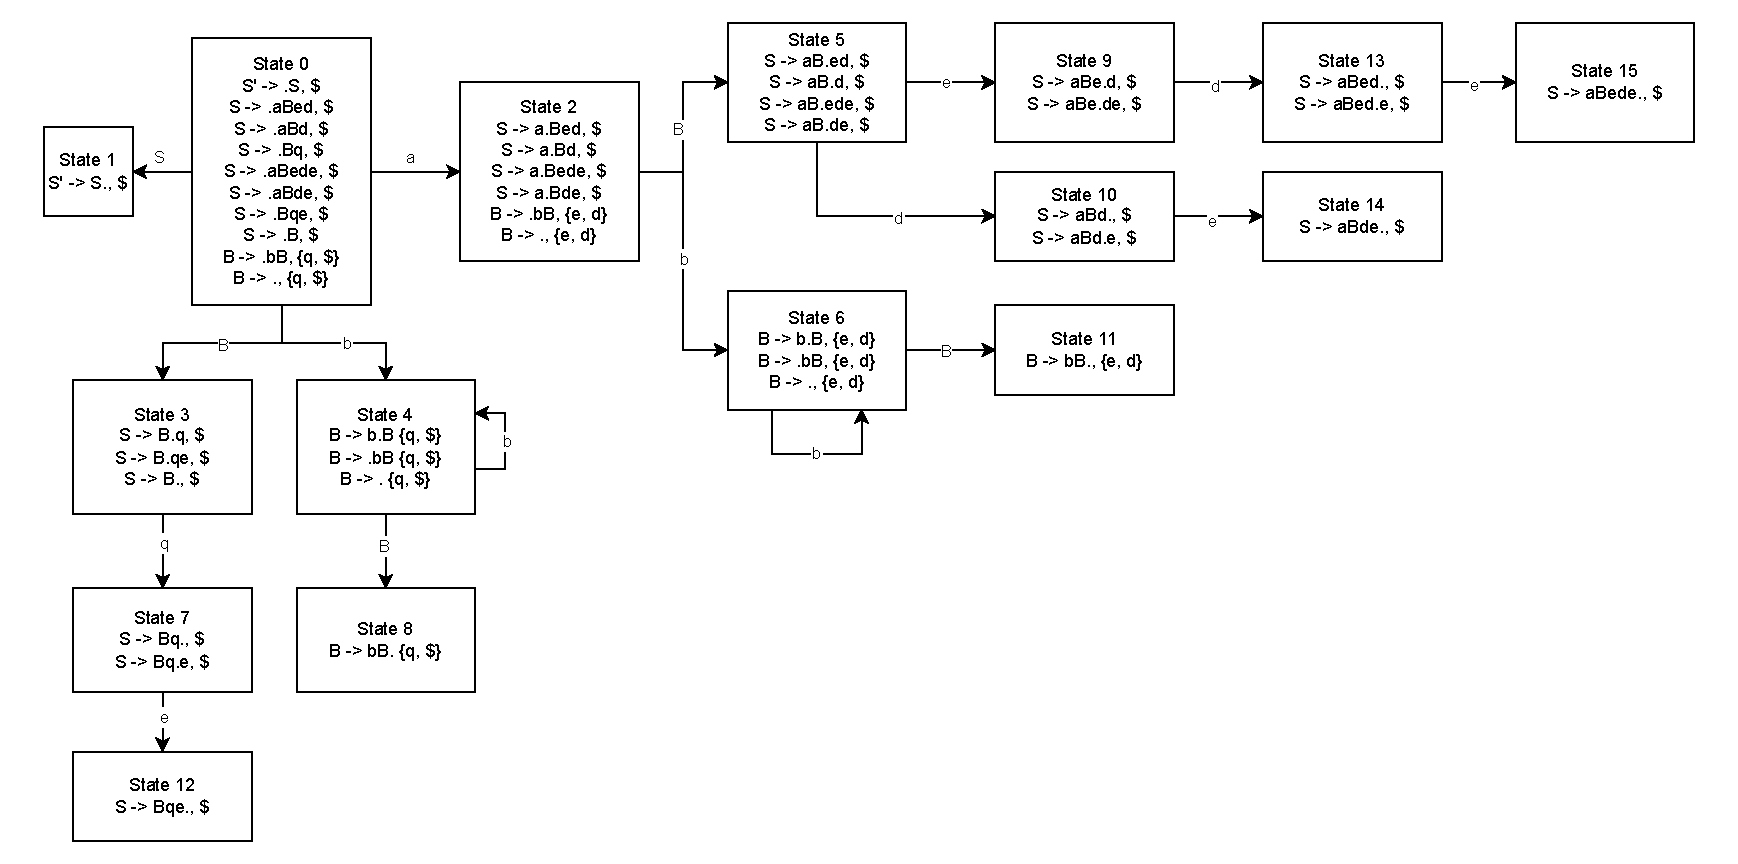
\includegraphics[width=1\textwidth]{figure/Q3-LR.pdf}
\end{figure}
\end{document}
